\documentclass[
%  master,
%  field=inf,
%  printversion,
%  biblatex,
%  language=czech,
%  font=sans,
  glossaries,
%  index
]{kidiplom}

\title{Domácí cloudové úložiště}
\title[english]{Home cloud storage}
\author{Aleš Kašpárek}
\supervisor{Mgr. Jan Tříska, PhD.}
\yearofsubmit{2021}
\annotation{Cílem práce je navrhnout a implementovat efektivní způsob uložení a sdílení souborů mezi uživateli, bez potřeby fyzického úložiště. Výsledkem práce je systém, pomocí kterého mohou uživatelé přistupovat ke svým souborům kdekoliv pomocí internetu.}
\annotation[english]{The main goal of thesis is to desing and implement efective way of storing and sharing files between users, without need of physical storage. Result of this thesis is a system, which allows users to use their files anywhere using the internet.}
\keywords{ cloud, cloudové úložiště, REST API, Python, GUI, C++, Docker}
\keywords[english]{cloud, cloud storage, REST API, Python, GUI, C++, Docker}
\thanks{Chtěl bych poděkovat Mgr. Janu Třískovi, PhD. za připomínky, nápady a zájem při tvoření této práce.}
\usepackage{lipsum}
\usepackage{float}

\begin{document}
\maketitle

\section{Úvod}
\label{sec:intro}
Cloud je v dnešní době velice oblíbené téma. Cloud lze popsat jako poskytování služeb nejčastěji dostupné přes prohlížeč nebo specializované aplikace, ke kterému lze přistupovat odkudkoliv po internetu. Cloud, jako služba taková, je provozována na virtualizovaném počítači, lokalizovaný na výkonných vzdálených serverech. Uživatel si poté pronajímá výkon těchto serverů. V dnešní době už u mnoha firem nenajdeme rozsáhlá IT oddělení a přecpané serverovny, protože je pro ně mnohem pohodlnější pronajmout si výpočetní sílu cloudu. Mezi základní výhody patří:
\begin{itemize}
\item škálovatelnost,
\item aktuálnost software,
\item "pay as you go" cenový model (platíme jen za to, co potřebujeme),
\item přístup po internetu \cite{WIKI_CLOUD}.
\end{itemize}
Distribuční model, který vypovídá o poskytovaných službách, obsahuje:
\begin{itemize}
\item IaaS - infrastruktura jako služba (servery a virtuální počítače (VM), úložiště, sítě a operační systémy),
\item Paas - platforma jako služba ( doručují na vyžádání prostředí pro vývoj, testování, doručování a správu softwarových aplikací),
\item SaaS - software jako služba (metoda doručování softwarových aplikací přes internet) \cite{MS_CLOUD}.
\end{itemize}

\subsection{Motivace}
Uložení dat a souborů v cloudu je jistě pohodlnější, než mít nestále po ruce fyzické úložiště. Jednak z hlediska sdílení mezi uživateli, tak z hlediska dostupného místa, kdy se uživatel nemusí obávat, zda-li ho má dost. 

Toto téma jsem si vybral z mnoha důvodů. Prvním důvodem je, že do cloudu se bude přesouvat stále více aplikací, a dál poroste. Dalším důvodem je moje zaměstnání, kde se zabývám vývojem aplikace pro cloud. Posledním důvodem, proč jsem zvolil toto téma, byla snaha vytvořit aplikaci, která umožní rychlé sdílení souborů v rámci naší rodiny.

\clearpage
\section{Stávající cloudová řešení}
Většina stávajících řešení je zpoplatněná metodou předplatného. Za tuto cenu pak nabízejí různou velikost úložiště, kterou může využívat. Řada těchto služeb poskytuje i možnost bezplatného používání, uživatelé jsou však v rámci této možnosti omezeni velikostí místa, které mohou využít. V rámci bezplatného používání se velikost použitelného místa pohybuje v rámci jednotek gigabajtů, nejvíce pak 15 GB, placení uživatelé pak mohou využívat místo v řádech terabajtů.

\subsection{Google Drive}
Tato služba je přirozenou volbou pro vlastníky zařízení Android, ve kterých je služba integrována, ostatní uživatelé pak ocení 15 GB prostoru. \cite{CLOUDSOLUTIONS} \textit {(volný překlad)}

S aplikací Google Photos pak mohou uživatelé se zařízením Android ukládat neomezené množství fotografií ve vysoké kvalitě. Po vylepšení na placený Google Drive uživatelé získají 2 TB místa, se kterým mohou pracovat, za cenu 99,99\$ ročně, a připojí se ke službě Google One. \cite{CLOUDSOLUTIONS} \textit {(volný překlad)}

Funkce poskytující Google Drive službou One, která se pojí k platformě Google Cloud, se neustále vyvíjí. \cite{CLOUDSOLUTIONS} \textit {(volný překlad)}

Mezi výhody této služby tak patří integrovaná podpora u zařízení s operačním systémem Android, štědrá nabídka úložného prostoru pro neplatící uživatele, a neomezený počet zařízení spjatých s jedním účtem.

Nevýhody zahrnují složité webové rozhraní, uživatelé operačních systémů Windows a Mac si pak mohou stáhnout desktopovou aplikaci, která jím umožní nahrávat soubory přetažením. \cite{CLOUDSOLUTIONS} \textit {(volný překlad)}

\subsection{Microsoft OneDrive}
Podobně jako Google Drive zaměřený na uživatele Googlu, OneDrive je mířený na uživatele Microsoftu, elegantní integraci s Outlook.com, populární emailovou platformou od této společnosti. \cite{CLOUDSOLUTIONS} \textit {(volný překlad)}

OneDrive se také váže s Windows 10 a také s celou řadou mobilních aplikací, umožňující přístup k souborům téměř odkudkoliv. Je také integrován se službami, které neposkytuje Microsoft, například s designovým gigantem AutoCAD. \cite{CLOUDSOLUTIONS} \textit {(volný překlad)}

Nabízí možnost sdílet soubory mezi uživateli, dokonce s uživateli, kteří sami nepoužívají OneDrive, a také možnost upravovat soubory online, bez nutnosti je stahovat. \cite{CLOUDSOLUTIONS} \textit {(volný překlad)}

OneDrive pocházející od společnosti Microsoft, spolčenosti s dostatkem peněz, je trochu zklamáním, že tato služba nabízí pro neplatící uživatele pouze 5 GB místa, ale od 2\$ měsíčně mohou uživatelé upgradovat na 100 GB. \cite{CLOUDSOLUTIONS} \textit {(volný překlad)}

Pokud uživatel vlastní Microsoft 365, dříve známý jako Office 365, získává k němu automaticky 1 TB úložiště s bezplatnou možností dalšího škálování. Musí mít však na paměti že se jedná pouze o úložný prostor bez jakýchkoliv dalších pokročilých funkcí. \cite{CLOUDSOLUTIONS} \textit {(volný překlad)}

Za 79.99\$ ročně pak mohou uživatelé přejít na placený plán pro 6 uživatelů, který nabízí 6 TB místa na osobu, tedy 1 TB na osobu. V rámci tohoto balíčku jsou zahrnuty další aplikace, například Word, Excel, a další. \cite{ONEDRIVE}

\subsection{Dropbox}
Při porovnání s podobnými službami, Dropbox podporuje relativně velký počet platforem od desktopu až po mobilní telefony. Nabízí celkem 10 klientů pro tyto platformy: Microsoft Windows, Mac OS a Linux (oficiální i neoficiální) a také pro oblast chytrých mobilních telefonů platforem Android, iPhone, iPad a BlackBerry. Důležitým prvkem Dropboxu je také webové rozhraní služby pro ty, kteří nemají nainstalovaného klienta. Dropbox používá model financování Freemium, což znamená, že v základním provedení je zdarma a poskytuje nenáročným uživatelům 2GB úložiště s omezením datových přenosů na 20 GB za den. U placených účtů je tento limit navýšen 2 TB úložiště a 200 GB přenosů za den. \cite{DROPBOX}

Zatímco Dropbox funguje i jako úložiště souborů, je zejména zaměřena na jejich synchronizaci a sdílení. Podporuje historii revizí, takže smazané soubory ze složky Dropbox mohou být kdykoliv obnoveny, a to jak přes webového klienta, tak i na kterémkoliv instalovaném klientu. Historie verzí je omezena na dobu 30 dní, ale uživatelé mají možnost získat neomezenou historii zakoupením placené verze. Dojde-li ke změně souboru v synchronizované Dropbox složce, automaticky dojde k synchronizaci na ostatní synchronizovaná zařízení. Výhodou Dropboxu je, že synchronizuje pouze tu část souboru, která se změnila, tak omezuje využívání internetu na minimum. \cite{DROPBOX}

Základní platební plán pro jednotlivce vyjde na 9,99€ měsíčně, a obsahuje již zmíněné 2 TB (2000 GB) úložiště pro jednoho uživatele, nabízí a stejně jako bezplatný plán nabízí 30denní obnovu souborů a historii verzí. Rodinný plán poté 16,99€, umožňuje přístup 6 uživatel, ale stále nabízí 2 TB prostoru a obsahuje také stejnou 30denní obnovu souborů a historii verzí. \cite{DROPBOXPRICE}

\subsection{IDrive}
IDrive nabízí synchronizaci souborů, dokonce i souborů na síťových discích. Webové rozhraní umožňuje sdílení přes email, Facebook a Twitter. Opatrní uživatelé rádi uslyší, že smazání souboru z počítače neznamená smazání souboru ze serveru, to znamená menší nebezpečí náhodného smazání něčeho důležitého. \cite{CLOUDSOLUTIONS} \textit {(volný překlad)}

Je zachováno až 30 předešlých verzí souborů na uživatelově účtu. Další věc, kterou je třeba poznamenat, je, že správci mají přístup k aplikaci IDrive Thin Client, která jim umožňuje zálohovat a obnovovat, spravovat nastavení, atd. pro všechny jejich připojené počítače prostřednictvím centralizovaného řídicího panelu. \cite{CLOUDSOLUTIONS} \textit {(volný překlad)}

Pro fotografie nabízí funkci rozpoznání obličeje, které pomáhá při organizaci fotografií. IDrive také nabízí službu IDrive Express, která uživateli v případě ztráty dat nabízí zaslání fyzického pevného disku, umožňující rychlé obnovení zálohovaných souborů. \cite{CLOUDSOLUTIONS} \textit {(volný překlad)}

IDrive nabízí hned několik možností předplatného. Základní bezplatná plán nabízí 5 GB využitelného místa. Další nabídka je 5, popř 10 TB, které stojí 52,12\$, popř. 74,62\$, nabízí přístup pro jednoho uživatele z neomezeného množství počítačů. Další plán začíná s přístupem z 5 počítačů, 5 TB místa a přístupu 5 uživatelů a škáluje až na 50 počítačů a uživatelů a 50 TB prostoru a začíná na 74,62\$. Poslední nabídka také obsahu hned několik nabídek různých velikostí úložiště, k tomu nabízí neomezený počet uživatelů, počítačů a serverů, mimo jiné také službu Exchange, SQL a také synchronizaci souborů na síťových discích a začíná na 74,62\$. \cite{IDRIVEPRICE}

\subsection{Backblaze}
Backblaze je gigant v odvětví cloudových úložišť, průmyslový veterán, který se stará jak o osobní, tak o velké obchodní zálohy. Klíčové slovo je zde \uv{záloha}, jelikož nenabízí žádnou synchronizaci ani kolaboraci. Backblaze nabízí zálohu, to je vše. Jako jediný nabízí skutečné neomezené cloudové úložiště, bez jakýchkoliv dalších závazků. \cite{CLOUDSOLUTIONS} \textit {(volný překlad)}

Cena předplatného pro osobní zálohy, která může být placena měsíčně, ročně, nebo v období 2 let, je velice výhodná (60\$ za rok), zvláště bereme-li v úvahu neomezenou velikost úložiště. \cite{CLOUDSOLUTIONS} \textit {(volný překlad)}

Mezi výhody Backblaze tedy patří neomezená velikost úložiště, společně při nákupu s ExpressVPN pak nízká cena, a jednoduchost. Oproti tomu na rozdíl od předchozích zmíněných řešení nenabízí kromě zálohování žádnou jinou funkci a uživatelům umožňuje přístup pouze z jednoho počítače. \cite{CLOUDSOLUTIONS}

\subsection{pCloud}
Tato služba jako jedna z mála nabízí možnost doživotního předplatného, v podstatě uživatel získá permanentní virtuální cloudovou jednotku. Služba se popisuje jako \uv{osobní cloudový prostor, kde můžete ukládat všechny svoje soubory a složky s uživatelsky přívětivým rozhraním které jasně ukazuje kde se všechno nachází a co dělá.} \cite{CLOUDSOLUTIONS} \textit {(volný překlad)}


pCloud nabízí 30 denní historii koše a neomezenou rychlost nahrávání, uživatelé jsou však omezeni velikostí stahování: 500 GB pro Premium a 2 TB pro Premium Plus za měsíc. \cite{CLOUDSOLUTIONS} \textit {(volný překlad)}

Od srpna 2020 také umožňuje uživatelům vybrat, zda-li chtějí mít svoje data uložená na serverech v Evropě nebo v Americe. Společnost samotná je registrovaná na Švýcarsku, které má přísné zákony pro soukromí, a proto nabízí možnost zaplatit 4,99\$ měsíčně za pCloud Crypto k zamčení (a odemčení) jednotlivých souborů heslem. \cite{CLOUDSOLUTIONS} \textit {(volný překlad)}

pCloud nabízí dvě možnosti předplatného. Patří sem služba Premium, která nabízí 500 GB prostoru, sdílení mezi uživateli, a 30 denní koš, za cenu 47,88€ ročně, nebo 175€ jednorázově na doživotí. Druhou možností je Premium Plus, nabízející 2 TB, a také sdílení a 30 denní koš. Za tuto možnost uživatelé zaplatí 95,88€ ročně, nebo 350€ jednorázově. \cite{PCLOUD}

\clearpage
\section{Použité technologie}
Aplikace je založena na komunikaci klienta se serverem, proto bylo velice důležité vybrat nástroj, který umožní snadný a rychlý vývoj serveru a jeho následné nasazení, stejně tak jako prostředek pro vývoj klientské aplikace, který jí umožní běžet jak na platformách Windows, tak na platformách Linux. Další nedílnou otázkou bylo zajištění hardwaru pro server. Po krátkém rozmýšlení padlo rozhodnutí na Raspberry Pi 4, které nabízí přijatelný výkon za nízkou cenu. Samotný server je kontejnerizován a nasazen pomocí nástroje Docker.

\subsection{Server}
Hlavními kritérii pro výběr technologie pro server byla snadná manipulace s HTTP požadavky, jednoduché sestrojení REST API, které funguje na výše zmíněném HTTP protokolu, jednoduchá práce s JSON soubory. Neméně důležitým kritériem byla moje znalost tohoto nástroje.

Vedlejšími faktory při výběru byly: jednoduchá práce s databází, podpora frameworku Swagger pro jednoduchý vývoj REST API, a nezávislost na operačním systému. Nakonec jsem zvolil Python s balíčkem connexion.

\subsubsection{Docker}
Docker je open-source platforma pro vývoj, nasazení a spouštění aplikací. Umožňuje zabalit a spustit aplikaci 	ve volně izolovaném prostředí nazývaném kontejner. Izolace a zabezpečení umožňuje běh několika kontejnerů najednou. Kontejnery jsou nenáročné a obsahují vše potřebné pro běh aplikace a na rozdíl od virtuálních strojů, které vyžadují hypervisor, jsou spuštěny přímo v rámci kernelu operačního systému.\cite{DOCKER} \textit {(volný překlad)}
\begin{figure}[htp]
    \centering
    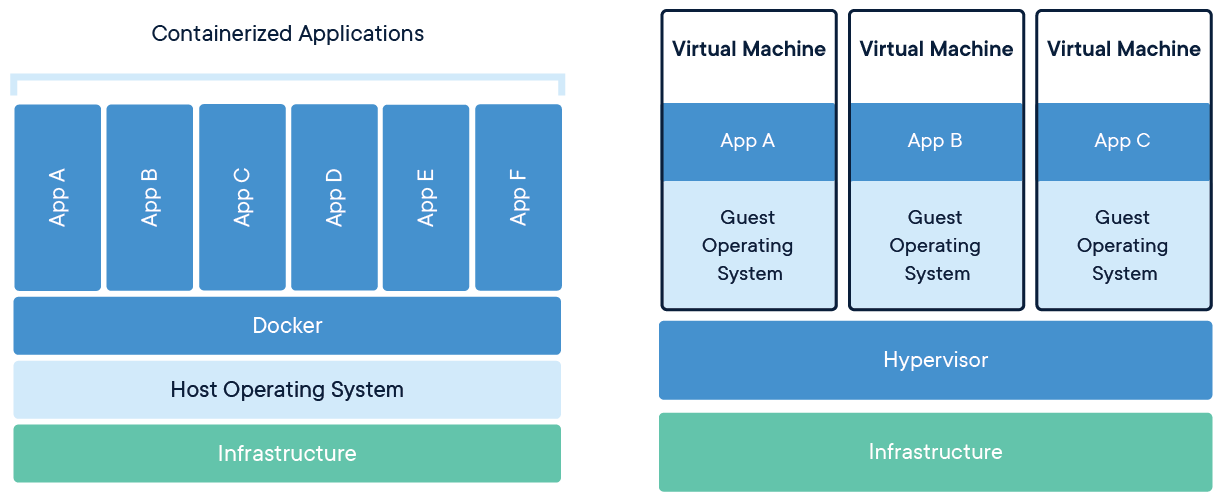
\includegraphics[width=10cm]{Docker-containerized-and-vm-transparent-bg}
    \caption{Srovnání dockeru a virtuálních strojů \cite{DOCKERIMAGE}}
    \label{fig:DockerSchema}
\end{figure}

\clearpage

\subsubsection{Python/Connexion}
Python je interpretovaný, objektově orientovaný, vysokoúrovňový programovací jazyk s dynamickou kontrolou datových typů. Podporuje moduly a balíčky, které zvyšují modularitu programu a znovupoužitelnost kódu. \cite{PYTHON} \textit {(volný překlad)}

Connexion je framework postavený na Flasku, který automaticky zpracovává HTTP požadavky, definované použitím OpenAPI (dříve známé jako Swagger). Connexion umožňuje psát tuto specifikaci, a poté mapuje koncové body na pythonové funkce. Toto je rozdíl od ostatních nástrojů, které generují specifikace podle kódu. \cite{CONNEXION} \textit {(volný překlad)}


\begin{kicode}{tex}{code:EndpointExample}{Ukázka endpointu}
paths:
  /apistatus:
    get:
      tags: 
        - API management
      summary: Health status of application
      description: Checks database availability and API response threshold time.
      operationId: manager.api_status.ApiStatus.get
      responses:
        200:
          description: API is healthy
        400:
          description: API is down
\end{kicode}

\subsection{Klientské části}
Dalším a neméně důležitým cílem bylo vytvoření aplikace, která bude spustitelná na počítačích s operačními systémy Windows a Linux. Jelikož jsem chtěl zabránit psaní dvou různých kódů pro obě tyto platformy, rozhodl jsem se využít frameworku Qt, který umožňuje vývoj aplikací s uživatelským rozhraní v jazyce C++.

Jelikož však C++ v základu neposkytuje tvorbu HTTP požadavků, práci se soubory ve formátu JSON, ani deterministickou hashovací funkci, proto bylo potřeba vybrání knihoven, které tuto funkčnost poskytnou.

\subsubsection{C++}
C++ je univerzální multiparadigmatický programovací jazyk vytvořený jako rozšíření programovacího jazyka C. Jazyk postupem času narostl, a moderní C++ je nyní objektově orientované, generické, má funkcionální rysy spolu s nízkoúrovňovou správou paměti. Téměř vždy je implementován jako kompilovaný jazyk. \cite{C++} \textit {(volný překlad)}


Bylo však nutné do standartní knihovny přidat další funkcionalitu zajišťující:
\begin{itemize}
\item Vytváření HTTP požadavků - knihovna libcurl, vývojová knihovna nástroje curl \cite{LIBCURL}.
\item Manipulaci s JSON soubory - knihovna nlohmann/json, přidává podporu pro manipulaci s JSON objekty podobnou jazyku Python \cite{JSONCPP}.
\item Deterministickou hashovací funkci - openssl, implementace protokolů SSL a TLS \cite{OPENSSL}.
\end{itemize}
S pomocí těchto nástrojů bylo možné se pustit do samotného vývoje.

\subsubsection{Qt}
Qt je multiplatformní framework široce používaný pro vytváření aplikací s grafickým uživatelským rozhraním určeným pro rozličné softwarové a hardwarové platformy. Qt je knihovna programovacího jazyka C++, ale existuje i pro jazyky Python (PyQt, PySide), Ruby (QtRuby), C, Perl, Pascal, C\#, Java (Jambi) a Haskell. Velkou výhodou Qt je velmi přehledně zpracovaná dokumentace a také vývojové programy Qt Creator nebo Qt Designer. Aplikace vytvořené pro grafické uživatelské prostředí používají nativní vzhled operačního systému, takže vyvinuté aplikace se vždy přizpůsobí vzhledu používaného prostředí \cite{QT}.

\clearpage
\section{Server}
Tato část se věnuje struktuře serveru a její implementaci. 
\subsection{Integrace databáze}
Jako databáze byl vybrán dockerový image Postgres. Dále bylo nutné napojit samotný server k této databázi. K tomuto jsem použil pythonový balíček Peewee. Zároveň bylo nutné vyřešit čekání serveru na inicializaci databáze.

\subsubsection{Čekání na databázi}
Čekání na databázi zajišťuje vstupní bod, ve kterém běží smyčka dotazování se na databázi.
\begin{kicode}{bash}{code:WaitForDB}{Mechanismus čekání na databázi}
until python3 utils/wait_for_db.py -eq 0 ; do
    echo "Waiting for database to initialize"
    sleep 2;
done
\end{kicode}

\subsubsection{Databázové třídy}
Databázové třídy odrážejí strukturu datového modelu. Bylo nutné vybrat vhodné datové typy, vyřešit relace mezi tabulkami, a povinné a nepovinné parametry.
\begin{itemize}
\item Jméno tabulky určuje atribut table\_name metatřídy, od které je třída odvozena.
\item Identifikátorem záznamu jsem zvolil typ UUID, které slouží k jedinečné indentifikaci záznamu, a je automaticky generováno při každém zápisu. Kód ~\ref{code:model} na řádku 7.
\item Atributy, které mohou nabývat hodnoty NULL, mají argument null nastaven na hodnotu True, a naopak.
\item Cizí klíče jsou reprezentovány hodnotou ForeignKeyField, specifikovaný třídou do které odkazuje a sloupcem. Kód ~\ref{code:model} na řádku 16 a 17.
\end{itemize}

\clearpage

\begin{kicode}{python}{code:model}{Třída databázové tabulky}
class BaseModel(Model):

    class Meta:
        database = DB

class NtwUsers(BaseModel):
    id = UUIDField(primary_key=True)
    user_name = TextField(null=False, unique=True)
    passw = TextField(null=False, unique=False)

    class Meta:
        table_name = "ntw_users"
        schema = SCHEMA_NAME
        
class Share(BaseModel):
    from_user = ForeignKeyField(NtwUsers, to_field='id')
    to_user = ForeignKeyField(NtwUsers, to_field='id')
    directory = TextField(null=False)
    file_name = TextField()

    class Meta:
        table_name = "share"
        schema = SCHEMA_NAME
        primary_key = False
\end{kicode}

\subsubsection{Metatřída a základní model}
Všechny třídy reprezentující databázové tabulky dědí ze základní třídy. V této třídě je specifikováno, ke které databázi se vztahují. Zde je specifikován atribut database, který obsahuje samotné připojení k databázi, má nastavené přihlašovací jméno a heslo, a mimo jiné i seznam, který rozšiřuje používané typy záznamů, o záznamy definované programátorem. Tento seznam bylo nutné použít, jelikož Peewee v základu nenabízí pole typu UUID.

V metatřídách jednotlivých databázových tříd je poté je poté nastaveno několik dalších informací, například je zde definován název tabulky a schéma, ve kterém se tabulka nachází, nebo například je zde uveden záznam, že daná tabulka neobsahuje žádný primární klíč.

\clearpage

\subsection{Struktura API}
\begin{figure}[htp]
    \centering
    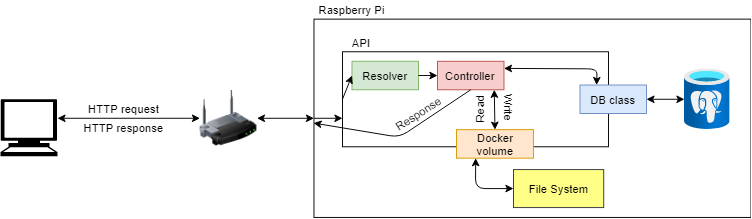
\includegraphics[width=15cm]{API_diagram}
    \caption{Schéma struktury API}
    \label{fig:APISchema}
\end{figure}

\subsubsection{Směřování}
Server ve výchozím nastavení naslouchá na portu 8000. Přístup zařízení, které se nachází ve stejné síti byl tento port zachován, ale pro zařízení, které se připojuje z jiné sítě, bylo nastaveno směřování portů z portu 80, na port 8000.

\subsubsection{API endpointy}
Endpointy definují samotnou strukturu API. Sestávají z metod, které obsluhují jednotlivé HTTP požadavky.
\begin{kicode}{python}{code:endpoint}{Ukázka endpointu}
class FilePostHandler(PostRequest):

    @classmethod
    def handle_post(cls, **kwargs):
        filePath = DISK_PATH + kwargs["user"] + kwargs["directory"]
        file = kwargs["fileName"]
        incomingFileSize = os.fstat(file.fileno()).st_size
        _, _, free = shutil.disk_usage(DISK_PATH)
        if incomingFileSize > free:
            return cls.format_exc("Internal server error", 500,"Not enough free space.") 
        savePath = filePath + str(unicodedata.normalize('NFKD', file.filename).encode('ascii', 'ignore'))[2:-1]
        file.save(savePath)
        return 200
\end{kicode}

Tento endpoint je definován pomocí OpenAPI následovně:

\begin{kicode}{python}{code:endpointDefinition}{Definice endpointu}
  /files/{user}:
    post:
      tags: 
        - File handling
      summary: Post a file.
      description: Post a file.
      operationId: manager.files.FilePostHandler.post
      ...
\end{kicode}


To, jaká metoda bude daný endpoint obsluhovat definuje atribut operationId na řádku 7 v ukázce ~\ref{code:endpointDefinition}. Endpoint pro  
~\ref{code:endpoint} obsluhuje požadavky na adrese 
\textit{[adresa\_serveru]/files/\{user\}}.

Protokol HTTP dovoluje použítí 8 \cite{HTTPmethods} metod, ale v práci jsem využil pouze 3 z nich, u jejich používání jsem dodržoval jejich definici.
\begin{itemize}
	\item GET- Tato metoda by měla pouze získávat data ze serveru.
	\item POST - Zasílání dat na server.
	\item DELETE - Smaže všechny výskyty zdroje z URI. 
\end{itemize}

Tento endpoint reaguje pouze na POST requesty, jak je možné vidět z řádku 2 v kódu 
~\ref{code:endpointDefinition}.

\subsubsection{Docker volume}
Volumes jsou preferovaným mechanismem pro persistenrní data generovaná a používaná kontejnery. \cite{DOCKERvolume} \textit {(volný překlad)}

Docker volume je jednoduchý nástroj kterým jsem docílil jednoduchého zapisování a odesílání souborů. Je velice snadné volume vytvořit za pomoci souboru docker-compose.yaml:
\begin{kicode}{python}{code:endpointDefinition}{Definice docker volume}
        volumes:
            - /media/pi/KINGSTON/NAS:/tmp/NAS
\end{kicode}
kde část před dvojtečkou odkazuje do souborového systému v rámci hostitelského systému, a část po dvojtečce udává, kde se v rámci kontejneru tyto soubory nachází. Jinými slovy to, co je v kontejneru uloženo v \textit {/tmp/NAS} bude fyzicky uloženo v \textit {/media/pi/KINGSTON/NAS}

\subsubsection{OpenAPI a dokumentace}
Nástroj OpenAPI (dříve známý jako Swagger), který automaticky zpracovává strukturu API z YAML souboru a poskytuje ji v podobě webové stránky a JSON souboru, jsem zvolil, jakožto nejjednodušší způsob udržování dokumentace. Vizuální dokumentaci API endpointu je možné vidět na obrázku ~\ref{fig:openapi}.


\begin{figure}[htp]
    \centering
    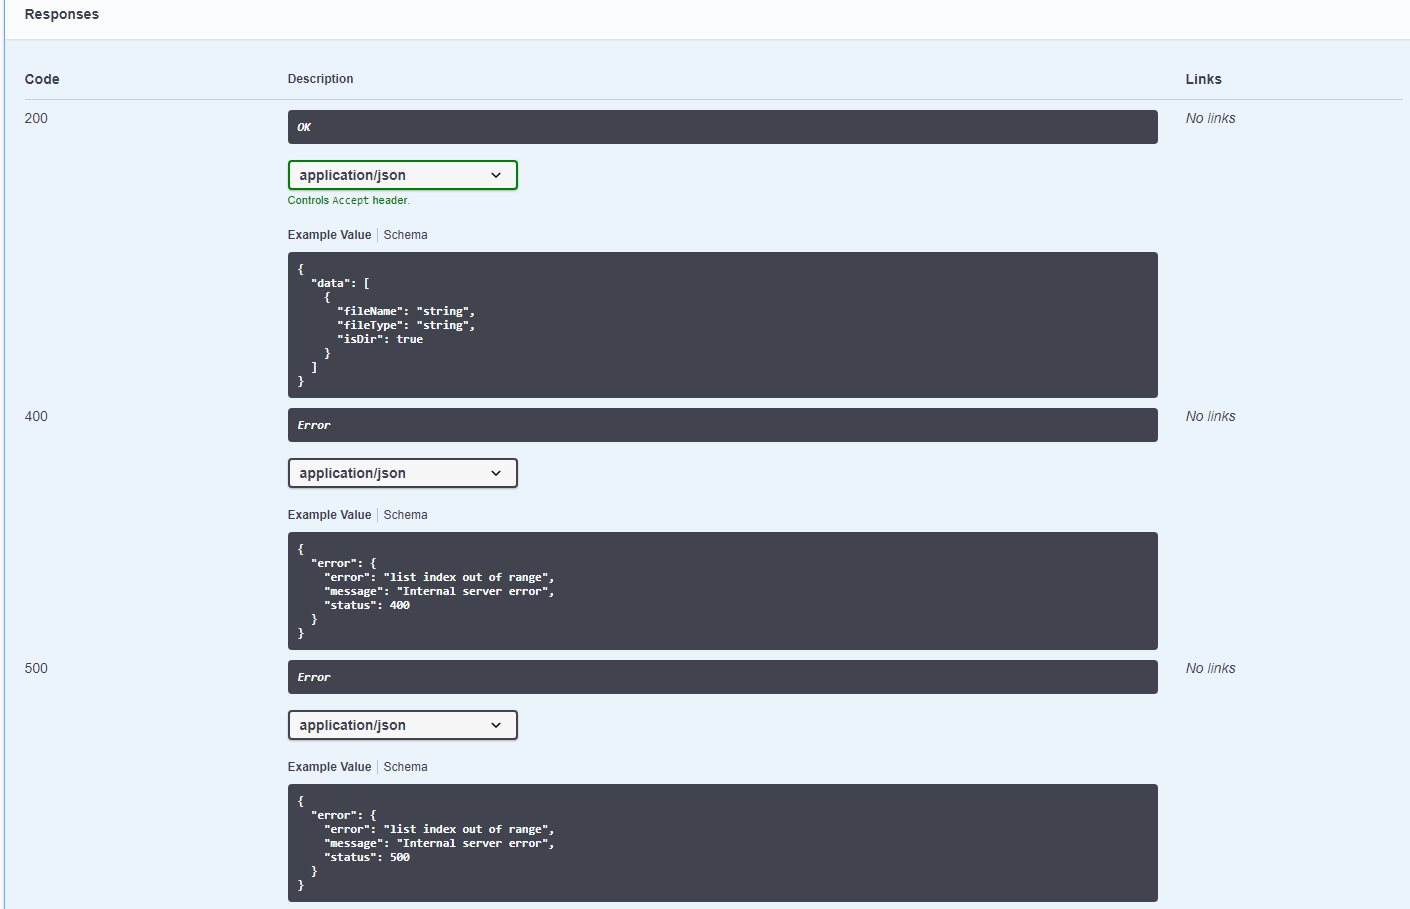
\includegraphics[width=14cm,height=10cm,keepaspectratio]{openapi}
    \caption{Ukázka grafické dokumentace OpenAPI}
    \label{fig:openapi}
\end{figure}
\clearpage
\subsubsection{Vývoj a debuggovací mód}
Jelikož server běží na Raspberry Pi, bylo žádoucí celý vývoj přesunout právě na něj, což však nebylo příliš komfortní. Právě proto nabízí Visual Studio Code rozšíření, které umožňuje využít protokolu SSH, a bylo možné tak pokračovat ve vývoji odkudkoliv.

Během vývoje bylo mnohokrát nutné některé endpointy složitě ladit. K ladění jsem využil balíček ptvsd, který implementuje debugger Visual Studia Code. Dále bylo nutné v rámci kontejneru povolit port 5678, na kterém tento debugger funguje a nastavení proměnné prostředí, která udává, zda-li se má server spustit v ladícím módu. Následně bylo nutné povolit debuggování v kódu, jak je ukázáno v ~\ref{code:debugMode}. Poslední požadavkem pro ladění bylo nakonfigurování Visudal Studia Code pro Python: Remote Attach. 
\begin{kicode}{python}{code:debugMode}{Zahájení debuggeru}
    if debug_mode:
        import ptvsd
        LOGGER.info("WAITING FOR DEBBUGER")
        ptvsd.enable_attach(address = ('0.0.0.0', 5678), redirect_output=True)
        ptvsd.wait_for_attach()
\end{kicode}
\clearpage
\section{Klientské části}
Tato část se věnuje implementaci uživatelské aplikace a také obsahuje uživatelskou dokumentaci.

\subsection{Dostupné platformy}
Aplikace byla vyvinuta a její zamýšlené nasazení se vztahuje na platformy Windows a Linux.

\subsubsection{Komunikace aplikace se serverem}
Veškerou komunikaci obstarává knihovna libcurl \cite{LIBCURL}, která zasílá požadavky na server, a přijímá odpovědi, které mohou být:
\begin{itemize}
	\item požadovaný soubor - v top případě je uložen do složky vytvořené v dočasných souborech následně v závislosti na platformě:
	\begin{itemize}
	\item Windows - je zavolána funkce \textit {ShellExecuteA} poskytovaná rozhraním Windows API, které požadovaný soubor otevře pomocí výchozí aplikace pro jeho otevření.
	\item Linux - je zavolána funkce \textit{fork}, která vytvoří nový proces, a v tomto procesu je provedeno volání \textit{execl} s argumentem \textit{"/usr/bin/xdg-open"}, a tento soubor je poté otevřen v tomto novém procesu opět pomocí výchozí aplikace.
	\end{itemize}
	\item JSON soubor - v tomto případě je odpověď parsována knihovnou nlohmann/json \cite{JSONCPP}, a poté zpracována.
\end{itemize}
\subsection{Uživatelská dokumentace}
\subsubsection{Dialog pro zadání IP adresy}
Při úplně prvním spuštění aplikace se uživateli zobrazí dialog pro zadání IP adresy zařízení, na kterém běží server a port. Uživatel je dotázán jak na adresu, kterou zařízení má ve stejné síti jako uživatel, a na veřejnou IP adresu. Je velice nutné, aby na routeru bylo nastavené směřování portů na port serveru a do příslušného zařízení. Uživatel je po potvrzení přesměrován na přihlašovací dialog. Pro účel této práce jsem přidal zaškrtávací políčko \textit{Use default}, které automaticky doplní adresu serveru běžícího na Raspberry Pi.
\begin{figure}[htp]
    \centering
    \includegraphics[width=8cm,height=7cm,keepaspectratio]{ip}
    \caption{Dialog pro zadání IP adres}
    \label{fig:ip}
\end{figure}
\subsubsection{Přihlašovací dialog}
Při každém dalším spuštění je uživateli ukázán jako první přihlašovací dialog. Zde si uživatel může buď vytvořit nový účet, nebo se přihlásit se stávajícím. Po potvrzení dialogu je zaslán požadavek na server o autorizaci uživatele. Během autorizace ještě na straně klienta dochází k použití algoritmu SHA-256 \cite{SHA256} z knihovny OpenSSL \cite{OPENSSL} k vytvoření hashe z hesla, jelikož hesla jsou v databázi uložena v hashované podobě. Poté je buď ukázána chybová hláška, že uživatel zadal špatné přihlašovací údaje, nebo dochází k zobrazení dialogu pro samotnou manipulaci se soubory.
\subsubsection{Uživatelské soubory}
\begin{figure}[htp]
    \centering
    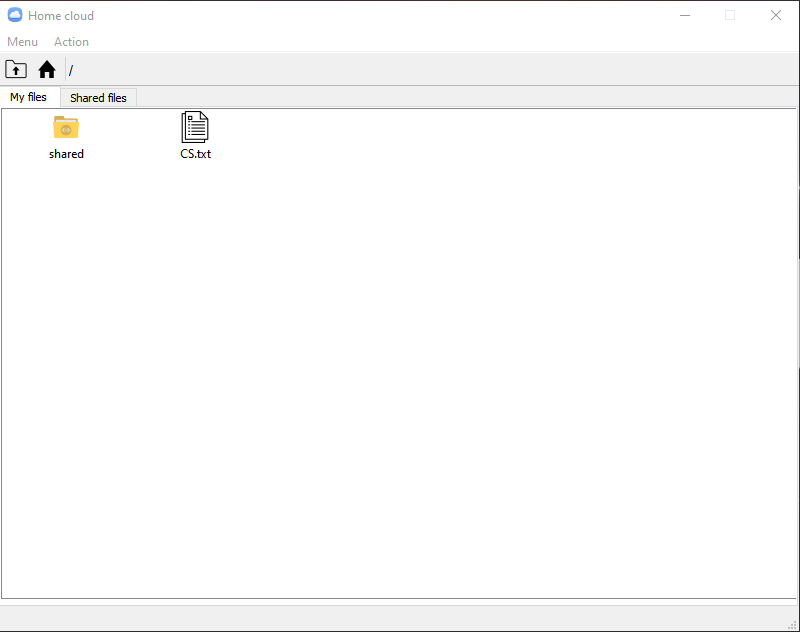
\includegraphics[width=14cm,height=10cm,keepaspectratio]{MainWindow}
    \caption{Uživatelova hlavní obrazovka}
    \label{fig:openapi}
\end{figure}
V hlavním okně má uživatel možnost procházet svoje soubory a soubory sdílené od ostatních uživatelů. Může také vytvořit složku kliknutím pravého tlačítka myši a vybráním možnosti \textit{Create folder}, nahrát nové soubory možností \textit{Upload file}, to samé může udělat buď z hlavní nabídky možností \textit{Action} a následně \textit{Upload}, nebo prostým přetáhnutím souboru, který chce nahrát.
\subsubsection{Sdílené soubory}
\begin{figure}[htp]
    \centering
    \includegraphics[width=14cm,height=10cm,keepaspectratio]{shared}
    \caption{Záložka se sdílenými soubory}
    \label{fig:shared}
\end{figure}
Uživatel může kdykoliv přepnout na záložku se soubory sdílených od ostatních uživatelů. Jako první si uživatel vybere od koho chce sdílené soubory zobrazit, a poté už vidí přímo sdílené soubory. Sdílet se mohou jak samostatné soubory, tak složky. Při sdílení složek dochází ke sdílení veškerého obsahu uvnitř složky. Když uživatel soubor smaže, dochází také automaticky k ukončení sdílení.
\subsection{Nasazení aplikace}
Aplikace je distribuována instalátorem. Pro tvorbu tohoto instalátoru jsem využil knihovnu Qt Installer Framework \cite{QTINSTALLER}. Tento framework umožňuje snadno a rychle vytvářet instalační soubory pro projety Qt, podporuje při tom platformy Microsoft Windows, Linux a macOS.
\clearpage
\section{Příručka vlastního spuštění server}
Jediným požadavkem pro spuštění serveru, je mít nainstalovanou službu Docker. Proto jsem do projektu přidal skript \textit{install.sh}, který tuto službu nainstaluje. Dále je nutný docker-compose, který tento skript také nainstaluje. K instalaci docker-compose je použit program pip, který, jelikož je server zamýšlen k nasazení výhradně na platformě Linux, je už předinstalovaný.

Druhý skript, \textit{start.sh}, poté slouží ke spuštění serveru.

\subsection{Statická IP adresa}
Uživatel by před samotným během serveru měl zajistit, aby stroji na kterém běží, byla přidělována statická IP adresa v rámci sítě. Tento krok je nezbytný jak v rámci přístupu v rámci domácí sítě, tak v rámci přístupu z jiného místa. Jelikož je nutné nastavení směřování portů, bez statické IP adresy by nemusely HTTP požadavky na server dorazit.

\subsection{Nastavení úložiště}
Nastavení úložiště se provádí nastavím docker volume, jak je možné vidět na řádku 2 v kódu ~\ref{code:endpointDefinition} v souboru \textit{docker-compose.yaml}. Uživatel pouze nastaví část před dvojtečkou na cestu, kam by chtěl, aby se mu soubory ukládaly.
\clearpage
\section{Možnosti dalšího vývoje}
Tento projekt zatím nabízí pouze uložení souborů, a do budoucna existuje celá řada vylepšení spousta dalších funkcí. 

Vytváření náhledových obrázků pro uložené soubory je první věcí, kterou bych chtěl do projektu představit. Tato změna bude představovat zjednodušení uživatelského rozhraní, jelikož se uživatelé ve svých souborech budou lépe orientovat pomocí právě těchto náhledů.

Dále bych chtěl umožnit streamování souborů ze serveru. Ať už jde o obrázky nebo videa, streamování je zajisté jednodušší než soubor stáhnout a poté ho otevřít. Dále bych chtěl představit možnost editovat soubory.

Do budoucna bych chtěl také přidat mobilní aplikaci, jak pro platformu Android, tak pro iOS, jelikož uživatelé budou chtít mít své soubory po ruce, i když zrovna nejsou u počítače.

Nakonec bych chtěl tento projekt udělat open-source, jelikož otevřený software nabízí neomezené množství nápadů a náhledů na tento projekt.

\begin{kiconclusions}
Cílem práce bylo vytvoření domácího cloudového úložiště a závěrečný program splňuje všechny tyto požadavky. Vytvořená aplikace je schopná běžet na obou hlavních platformách. Aplikace umožňuje snadný přístup k souborům uloženým na vzdáleném serveru, umožňuje správu uživatelů a sdílení souborů mezi těmito uživateli. 

Jelikož jsem před začátkem této práce neměl zkušenosti s návrhem a implementací takto rozsáhlého systému, tak dalším výsledkem této práce je právě tato zkušenost. Byl jsem schopen vyzkoušen návrh serverové architektury, návrh a implementace uživatelského rozhraní a také správu sítí. Jako největší přínos této práce vidím výslednou aplikaci, kterou hodlám používat a rozšířit v rodinném prostředí.

\end{kiconclusions}

\begin{kiconclusions}[english]
The main goal of this thesis was to create home cloud storage and the resulting program meets all the requirements. Created application is capable of running on both main platforms. Application allows easy way of accessing files on remote server, allows management of users and sharing files between this users.

Before I've started working on this theses, I've had no experience with desing and implementation of such an extensive system, the result of this thesis is this experience. I was able to try designing server architecture, design and implementation of user interface and network management. As the biggest benefit of this thesis I see the resulting application, which I intend to use and spread in family environment.


\end{kiconclusions}

\begin{thebibliography}{Cloud}
	\bibitem[1]{WIKI_CLOUD} Cloud computing - Wikipedie. [online]. Dostupné z: 
		\url{https://cs.wikipedia.org/wiki/Cloud\_computing}
	\bibitem[2] {MS_CLOUD} Co je cloud computing? Průvodce pro začátečníky | Microsoft Azure [online]. Dostupné z: 
		\url{https://azure.microsoft.com/cs-cz/overview/what-is-cloud-computing/\#cloud-computing-models}
	\bibitem[3]{DOCKER} Docker overview | Docker Documentation. [online]. Dostupné z:
		\url{https://docs.docker.com/get-started/overview/}
	\bibitem[4]{PYTHON} What is Python? Executive Summary | Python.org [online].
	Dostupné z:
		\url{https://www.python.org/doc/essays/blurb/}
	\bibitem[5]{CONNEXION} Welcome to Connexion’s documentation! — Connexion 2.0 documentation [online]. Dostupné z: 
		\url{https://connexion.readthedocs.io/en/latest/}
	\bibitem[6]{C++} C++ - Wikipedia [online]. Dostupné z:
		\url{https://en.wikipedia.org/wiki/C++}
	\bibitem[7]{QT} Qt (knihovna) – Wikipedie [online]. Dostupné z:
		\url{https://cs.wikipedia.org/wiki/Qt\_(knihovna)}
	\bibitem[8]{DOCKERvolume} Use volumes | Docker Documentation [online]. Dostupné z:
		\url{https://docs.docker.com/storage/volumes/}
	\bibitem[9]{HTTPmethods}  HTTP request methods - HTTP | MDN [online]. Dostupné z:
		\url{https://developer.mozilla.org/en-US/docs/Web/HTTP/Methods}
	\bibitem[10]{LIBCURL}  libcurl - the multiprotocol file transfer library [online]. Dostupné z:
		\url{https://curl.se/libcurl/}
	\bibitem[11]{JSONCPP}  nlohmann/json: JSON for Modern C++ [online]. Dostupné z:
		\url{https://github.com/nlohmann/json}
	\bibitem[12]{OPENSSL}  OpenSSL [online]. Dostupné z:
		\url{https://www.openssl.org/}
	\bibitem[13]{SHA256}  Secure Hash Algorithm – Wikipedie [online]. Dostupné z:
		\url{https://cs.wikipedia.org/wiki/Secure\_Hash\_Algorithm}
	\bibitem[14]{QTINSTALLER} Qt Installer Framework Manual [online]. Dostupné z:
		\url{https://doc.qt.io/qtinstallerframework/index.html}
	\bibitem[15]{DOCKERIMAGE} File:Docker-containerized-and-vm-transparent-bg.png - Wikimedia Commons [online]. Dostupné z:
		\url{https://commons.wikimedia.org/wiki/File:Docker-containerized-and-vm-transparent-bg.png}
	\bibitem[16]{CLOUDSOLUTIONS} Best cloud storage services for 2021 | TechRadar [online]. Dostupné z:
		\url{https://www.techradar.com/news/the-best-cloud-storage}
	\bibitem[17]{DROPBOX} Dropbox – Wikipedie [online]. Dostupné z:
		\url{https://cs.wikipedia.org/wiki/Dropbox}
	\bibitem[18]{ONEDRIVE} Cloud Storage Pricing and Plans – Microsoft OneDrive [online]. Dostupné z:
		\url{https://www.microsoft.com/en-ww/microsoft-365/onedrive/compare-onedrive-plans?market=af}
	\bibitem[19]{DROPBOXPRICE} Compare All Dropbox Plans ‐ Dropbox [online]. Dostupné z:
		\url{https://www.dropbox.com/plans?tab=personal}
	\bibitem[20]{IDRIVEPRICE} IDrive® pricing plans [online]. Dostupné z:
		\url{https://www.idrive.com/pricing}
	\bibitem[21]{PCLOUD} pCloud - Best Cloud Storage Pricing \& Cost Plans [online]. Dostupné z:
		\url{https://www.pcloud.com/cloud-storage-pricing-plans.html}
\end{thebibliography}
\clearpage

\appendix
\section{Obsah přiloženého CD/DVD} \label{sec:ObsahCD}
\begin{description}

\item[\texttt{desktop\_app/}] \hfill \\
 Složka s aplikací. Obsahuje instalační soubory pro Windows a Linux. Dále obsahuje zdrojový kód desktopové aplikace

\item[\texttt{server/}] \hfill \\
   Složka obsahující zdrojové kódy serveru.
   
\item[\texttt{theses/}] \hfill \\
Složka se textem práce a jeho zdrojovým kódem.

\item[\texttt{readme.txt}] \hfill \\
  Instrukce pro spuštění.
 

\end{description}

\end{document}